\documentclass[12pt, a4paper]{article}
\usepackage{../../../myconfig} % Gọi file cấu hình từ ngoài gốc vào

% ==========================================
% BẮT ĐẦU NỘI DUNG TÀI LIỆU
% ==========================================
\begin{document}

% Truyền 3 tham số: {Nhãn cam} {Chữ to chính giữa} {Chữ ở góc phải Header}
\titlebox{Chủ đề: Hàm số}{BT điểm danh đường tiện cận}{Hàm số: Đường tiện cận}

\questionLinesManual{4}{1}{Cho hàm số \( y = f(x) \) có bảng biến thiên như hình vẽ dưới đây.

\begin{center}

\begin{tikzpicture}
    \tkzTabInit[lgt=1.5, espcl=3.5]
    {$x$ /1, $y'$ /1, $y$ /2.5}
    {$-\infty$, $1$, $2$, $+\infty$}
    \tkzTabLine{, -, d, -, 0, +, }
    \tkzTabVar{+/ $-1$ / , -D+/ $-\infty$ / $+\infty$ , -/ $1$ / , +/ $2$ /}
\end{tikzpicture}
\end{center}

Đồ thị hàm số \( y = f(x) \) có bao nhiêu đường tiệm cận?}{
    \begin{tasks}(4)
        \task $3$
        \task $2$
        \task $1$
        \task $4$
    \end{tasks}
}

\questionLinesManual{4}{2}{Cho hàm số \( y = f(x) \) có bảng biến thiên như sau

\begin{center}

\begin{tikzpicture}
    \tkzTabInit[lgt=1.5, espcl=2.5]
    {$x$ /1, $y'$ /1, $y$ /2.5}
    {$-\infty$, $-2$, $0$, $+\infty$}
    \tkzTabLine{, -, d, +, d, -, }
    \tkzTabVar{+/ $+\infty$ / , -D-/ $1$ / $-\infty$/ ,+D+/ $+\infty$ / $1$ , -/ $0$ /}
\end{tikzpicture}
\end{center}

Tổng số đường tiệm cận đứng và tiệm cận ngang của đồ thị hàm số đã cho bằng}{
    \begin{tasks}(4)
        \task $3$
        \task $2$
        \task $1$
        \task $0$
    \end{tasks}
}

\questionLinesManual{4}{3}{Cho hàm số \( y = f(x) \) có bảng biến thiên như hình vẽ dưới đây. Hỏi đồ thị của hàm số đã cho có bao nhiêu đường tiệm cận?

\begin{center}
\begin{tikzpicture}
    \tkzTabInit[lgt=1.5, espcl=2.5]
    {$x$ /1, $y'$ /1, $y$ /2.5}
    {$-\infty$, $-2$, $0$, $+\infty$}
    \tkzTabLine{,,d, +, d, -,}
    \tkzTabVar{,D-// $-\infty$ / , +D+/ $+\infty$ / $1$ , -/ $0$ /}
    \fill[pattern=north east lines](1.5,-4.5) rectangle (4.5,-1);
\end{tikzpicture}
\end{center}

}{
    \begin{tasks}(4)
        \task $3$
        \task $2$
        \task $4$
        \task $1$
    \end{tasks}
}


\questionLinesManual{4}{4}{Cho hàm số \( y = \dfrac{ax + b}{cx + d} \) (\( c \neq 0, ad - bc \neq 0 \)) có đồ thị như hình vẽ bên. Tiệm cận đứng của đồ thị hàm số là:

\begin{center}
\begin{tikzpicture}[>=latex, scale=0.8]
    % 1. Hệ trục tọa độ
    \draw[->] (-3.5,0) -- (5.5,0) node[below] {\small $x$};
    \draw[->] (0,-4.5) -- (0,3.5) node[right] {\small $y$};
    \node[below left] at (0,0) {\small $O$};
    
    % 2. Vẽ đồ thị hàm số
    \draw[thick, samples=100, domain=-3.5:0.71] 
        plot (\x, {(-\x+2)/(\x - 1)});
    \draw[thick, samples=100, domain=1.22:5] 
        plot (\x, {(-\x+2)/(\x - 1)});
    % 3. Đường tiệm cận
    \draw[thick] (1,-4.5) -- (1,3.5);
    \draw[thick] (-3.5,-1) -- (3.5,-1) ;
    
    % 4. Đánh dấu các điểm
    \node[below left] at (1,0) {\small $1$};
    \node[below left] at (2,0) {\small $2$};
    \node[below left ] at (0,-1) {\small $-1$};
    \node[below left] at (0,-2) {\small $-2$};
    \filldraw (1,-2) circle (1.5pt);
    \filldraw (2,0) circle (1.5pt);
    \filldraw (0,-1) circle (1.5pt);
    \filldraw (0,-2) circle (1.5pt);
\end{tikzpicture}
\end{center}

}{
    \begin{tasks}(4)
        \task \( x = -1 \)
        \task \( y = -1 \)
        \task \( x = 1 \)
        \task \( y = 1 \)
    \end{tasks}
}

\questionLinesManual{4}{5}{Cho hàm số \( y = \dfrac{ax + b}{cx + d} \) (\( c \neq 0; ad - bc \neq 0 \)) có đồ thị như hình vẽ.

\begin{center}
\begin{tikzpicture}[>=latex, scale=0.6]
    % 1. Hệ trục tọa độ
    \draw[->] (-6.5,0) -- (6.5,0) node[below] {\small $x$};
    \draw[->] (0,-4.5) -- (0,6.5) node[right] {\small $y$};
    \node[below left] at (0,0) {\small $O$};
    
    % 2. Vẽ đồ thị hàm số
    \draw[thick, samples=100, domain=-6.5:-1.65] 
        plot (\x, {(2*\x - 1)/(\x +1)});
    \draw[thick, samples=100, domain=-0.54:6.6] 
        plot (\x, {(2*\x - 1)/(\x +1)});
    % 3. Đường tiệm cận
    \draw[thick] (-1,-4.5) -- (-1,6.5) ;
    \draw[thick] (-6.5,2) -- (6.5,2);
    
    % 4. Đánh dấu các điểm
    \node[right] at (0,-1) {\small $-1$};
    \node[above right] at (0,2) {\small $2$};
    \node[below left] at (-1,0) {\small $-1$};
    \filldraw (-1,0) circle (1.5pt);
    \filldraw (0,2) circle (1.5pt);
    \filldraw (0,-1) circle (1.5pt);
\end{tikzpicture}
\end{center}

Tiệm cận ngang của đồ thị hàm số đã cho là}{
    \begin{tasks}(4)
        \task \( x = 2 \)
        \task \( y = 1 \)
        \task \( y = 2 \)
        \task \( x = 2 \)
    \end{tasks}
}

\questionLinesManual{4}{6}{Cho hàm số \( f(x) = \dfrac{ax^2 + bx + c}{dx + e} \) (\( a, b, c, d, e \in \mathbb{R}, ad \neq 0 \)) có đồ thị như hình vẽ.

\begin{center}
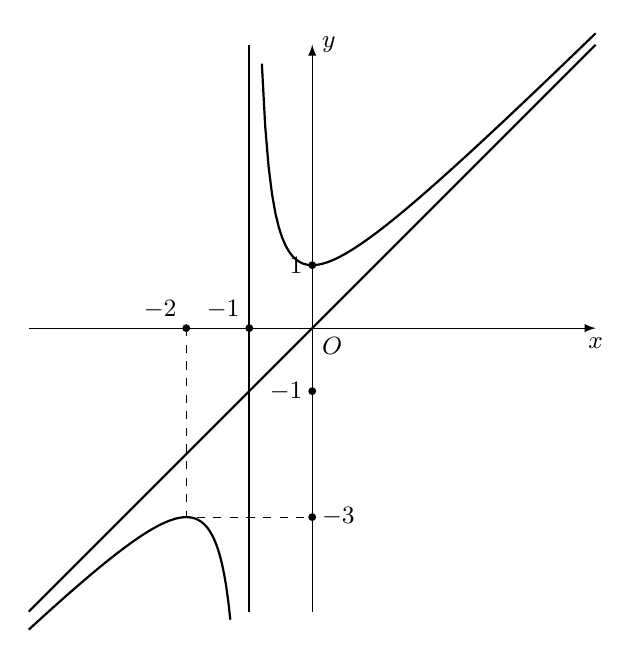
\begin{tikzpicture}[>=latex, scale=0.8]
    % 1. Hệ trục tọa độ
    \draw[->] (-4.5,0) -- (4.5,0) node[below] {\small $x$};
    \draw[->] (0,-4.5) -- (0,4.5) node[right] {\small $y$};
    \node[below right] at (0,0) {\small $O$};
    
    % 2. Vẽ đồ thị hàm số
    \draw[thick, samples=100, domain=-4.5:-1.3] 
        plot (\x, {\x + 1/(\x + 1)});
    \draw[thick, samples=100, domain=-0.8:4.5] 
        plot (\x, {\x + 1/(\x + 1)});
    \draw[thick, samples=100, domain=-4.5:4.5] 
        plot (\x, {\x});
    
    % 4. Đường tiệm cận đứng
    \draw[thick] (-1,-4.5) -- (-1,4.5) ;
    
    % 5. Đánh dấu các điểm
    \node[above left] at (-1,0) {\small $-1$};
    \node[left] at (0,1) {\small $1$};
    \node[right] at (0,-3) {\small $-3$};
    \node[above left] at (-2,0) {\small $-2$};
    \node[left] at (0,-1) {\small $-1$};
    \filldraw (-1,0) circle (1.5pt);
    \filldraw (0,1) circle (1.5pt);
    \filldraw (0,-3) circle (1.5pt);
    \filldraw (-2,0) circle (1.5pt);
    \filldraw (0,-1) circle (1.5pt);
    \draw[dashed] (-2,0)-- (-2,-3) -- (0,-3);
\end{tikzpicture}
\end{center}

Tiệm cận xiên của đồ thị hàm số đã cho là}{
    \begin{tasks}(4)
        \task \( y = -x \)
        \task \( y = x \)
        \task \( y = x - 1 \)
        \task \( y = x + 1 \)
    \end{tasks}
}

\questionLinesManual{4}{7}{Cho hàm số \( y = f(x) \) có đồ thị hàm số như hình sau:

\begin{center}
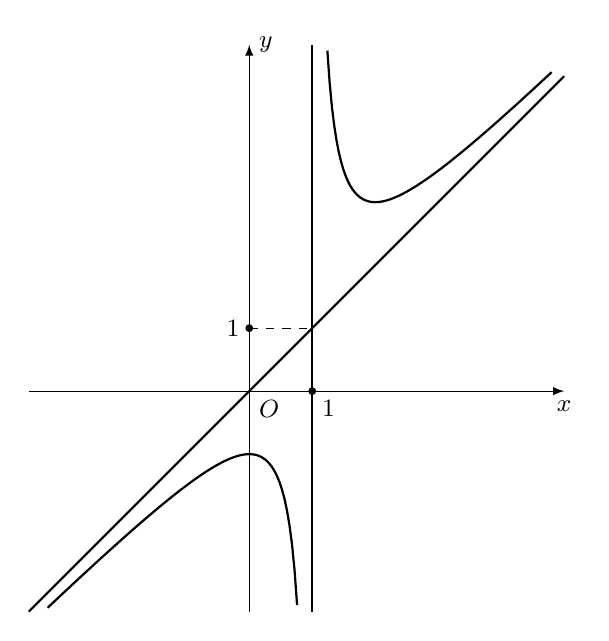
\begin{tikzpicture}[>=latex, scale=0.8]
    % 1. Hệ trục tọa độ
    \draw[->] (-3.5,0) -- (5,0) node[below] {\small $x$};
    \draw[->] (0,-3.5) -- (0,5.5) node[right] {\small $y$};
    \node[below right] at (0,0) {\small $O$};
    
    % 2. Vẽ đồ thị hàm số (có tiệm cận xiên y = x - 1)
    \draw[thick, samples=100, domain=-3.2:0.76] 
        plot (\x, {\x  + 1/(\x-1)});
    \draw[thick, samples=100, domain=1.24:4.8] 
        plot (\x, {\x  + 1/(\x-1)});
    \draw[thick, samples=100, domain=-3.5:5] 
        plot (\x, {\x  });
    % 4. Đường tiệm cận đứng
    \draw[thick] (1,-3.5) -- (1,5.5);
    \draw[dashed] (0,1)--(1,1);
    % 5. Đánh dấu các điểm
   
    \node[below right] at (1,0) {\small $1$};
    \node[left] at (0,1) {\small $1$};
    \filldraw (1,0) circle (1.5pt);
    \filldraw (0,1) circle (1.5pt);
\end{tikzpicture}
\end{center}

Đường tiệm cận xiên của đồ thị hàm số là}{
    \begin{tasks}(4)
        \task \( y = x - 1 \)
        \task \( y = 2 - x \)
        \task \( y = x \)
        \task \( y = x + 1 \)
    \end{tasks}
}

\questionLinesManual{4}{8}{Tiệm cận ngang của đồ thị hàm số \( y = \dfrac{4x + 1}{x - 1} \) là}{
    \begin{tasks}(4)
        \task \( y = \dfrac{1}{4} \)
        \task \( y = 4 \)
        \task \( y = 1 \)
        \task \( y = -1 \)
    \end{tasks}
}

\questionLinesManual{4}{9}{Đường tiệm cận xiên của đồ thị hàm số \( y = \dfrac{x^2 - 2x}{x + 1} \) có phương trình là}{
    \begin{tasks}(4)
        \task \( y = x - 1 \)
        \task \( y = x - 3 \)
        \task \( y = x + 1 \)
        \task \( y = x \)
    \end{tasks}
}

\questionLinesManual{4}{10}{Đường thẳng \( y = -2x + 1 \) là tiệm cận xiên của đồ thị hàm số nào dưới đây?}{
    \begin{tasks}(2)
        \task \( y = -2x + 1 - \dfrac{3}{x - 2} \)
        \task \( y = x + 1 + \dfrac{1}{-2x + 1} \)
        \task \( y = 3x - 2 + \dfrac{3}{2x - 1} \)
        \task \( y = \dfrac{1}{-2x + 1} \)
    \end{tasks}
}



\end{document}